\label{experiments}
Several dataset~\cite{ClusteringDatasets} are used in order to evaluate the correctness 
of this solution. This phase is a very important in order to understand its potentialities.

The assessment is performed using input data that have very different properties,
starting from one with many small and dense cluster and ending with a dataset with few 
but very sparse clusters. In this way it is possible to see how the implementation
behaves under very different scenarios.

\begin{figure}[t]
  \center{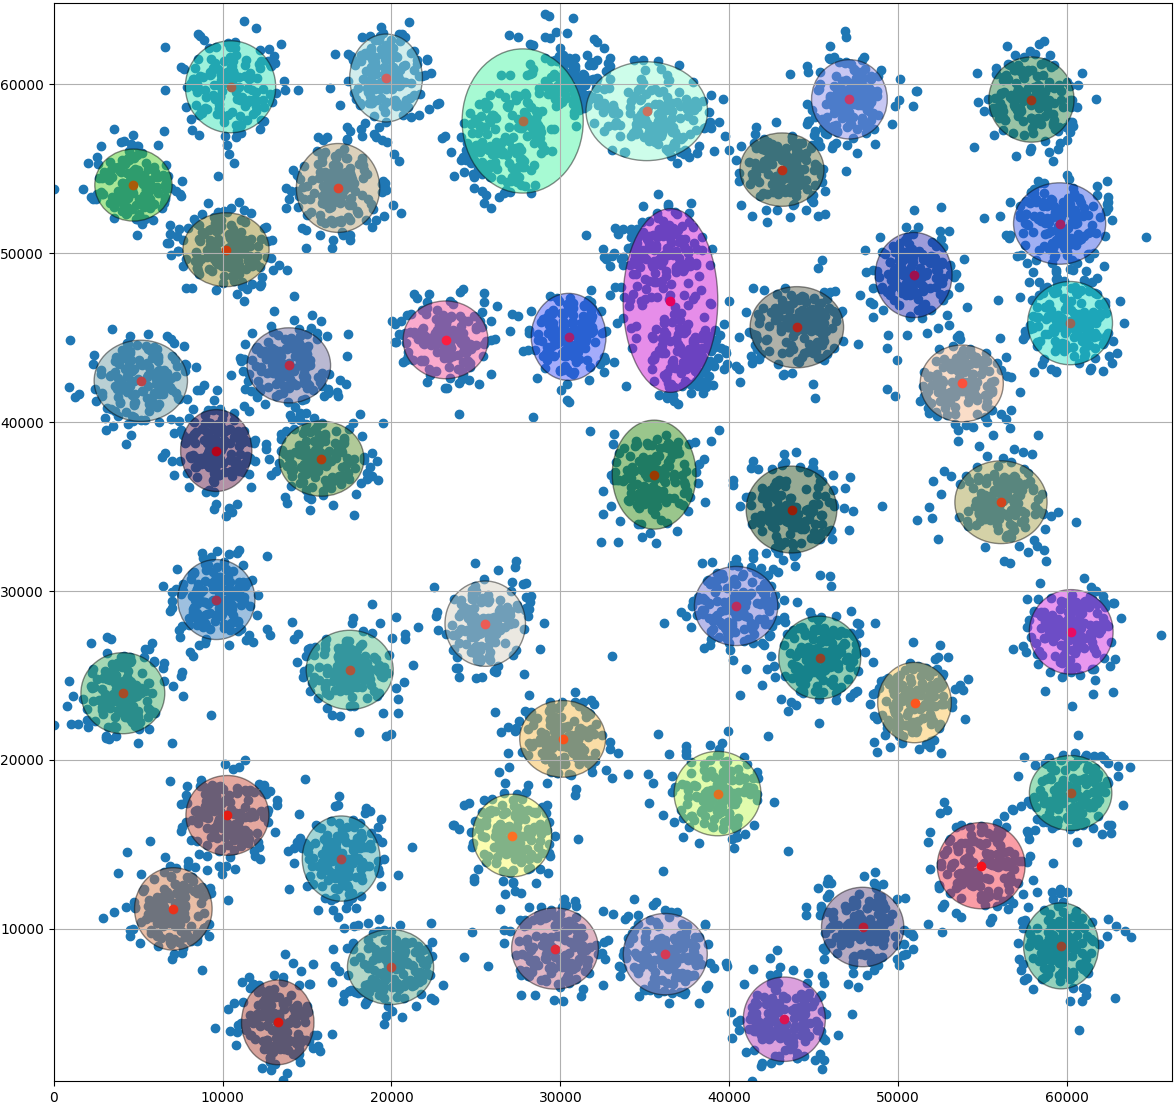
\includegraphics[width=0.5\textwidth]{a3_density_3.png}}
  \caption{The final outcome from a dataset with many small and dense regions.}
  \label{dataset1}
\end{figure}

\begin{figure}[t]
  \center{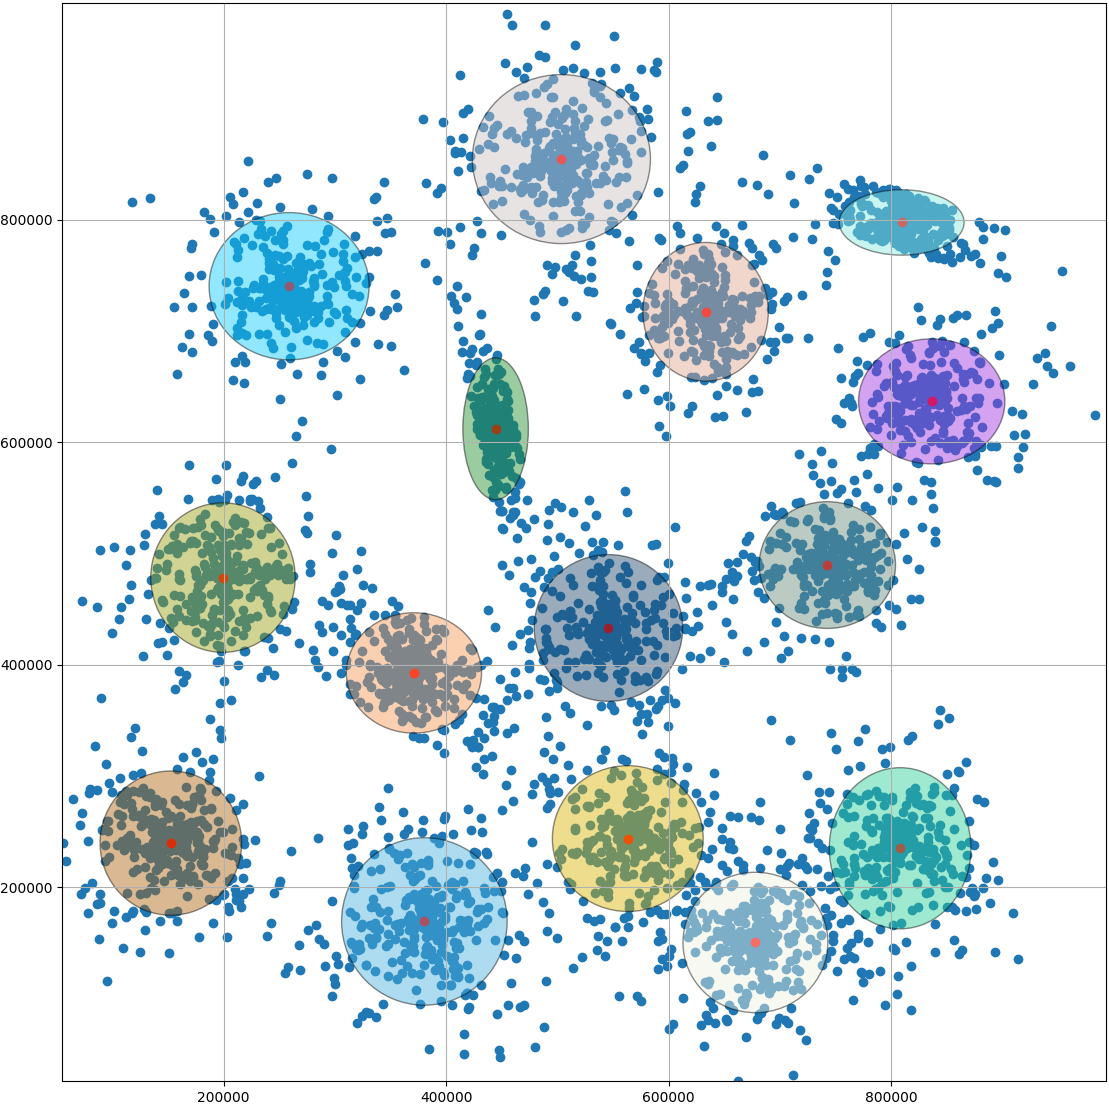
\includegraphics[width=0.5\textwidth]{s2_density_3.png}}
  \caption{The final outcome from a dataset with many small and quite sparse points.}
  \label{dataset2}
\end{figure}

\begin{figure}[t]
  \center{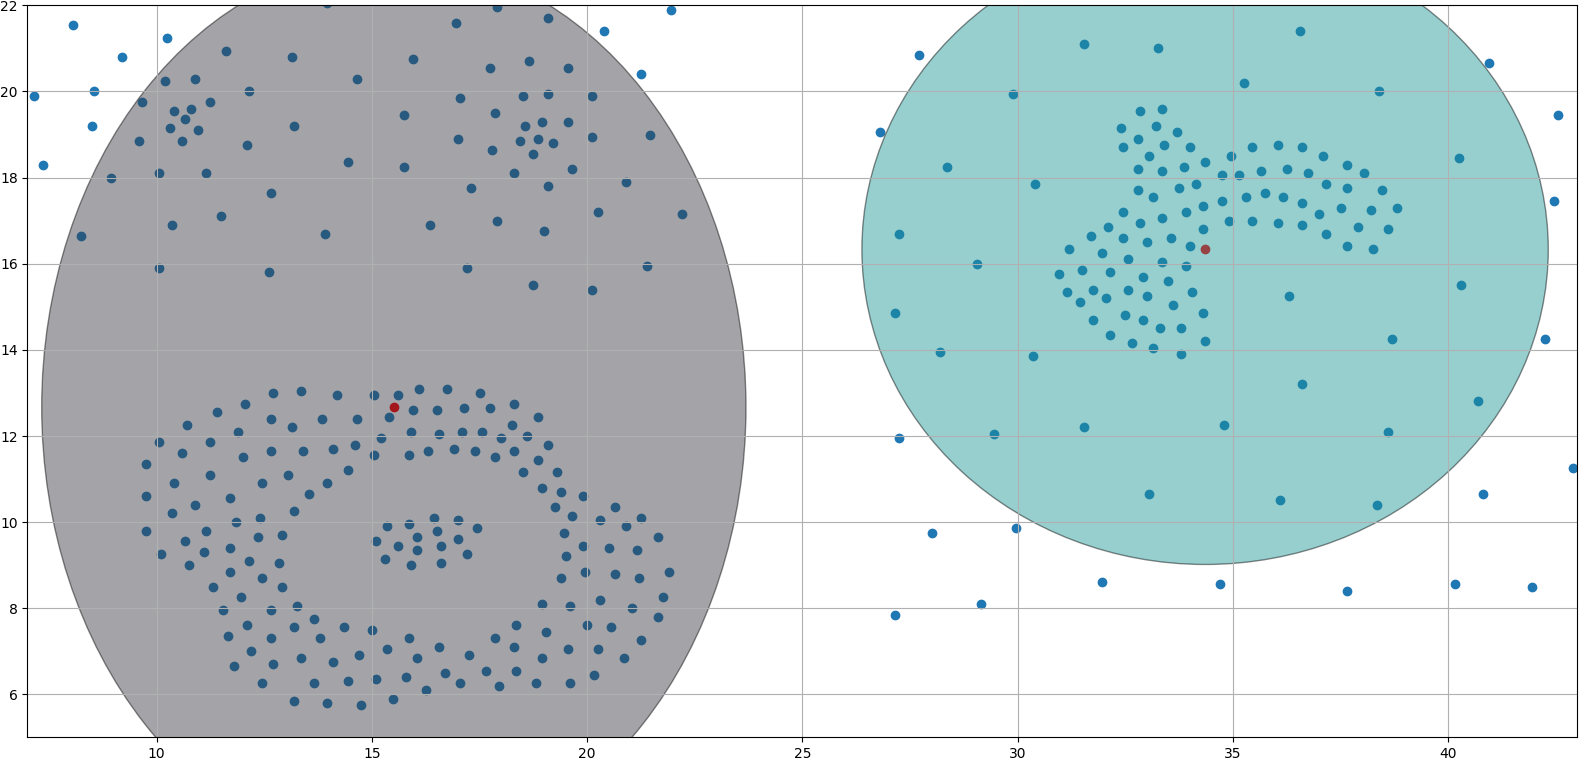
\includegraphics[width=0.5\textwidth]{Compound_density_1.png}}
  \caption{The final outcome from a very difficult dataset for a "k-means"-like algorithm.}
  \label{dataset3}
\end{figure}

As it is possible to see from Figure~\ref{dataset1} and \ref{dataset2}, this approach
succeeds both in finding the right number of clusters and in positioning the centroids, even
though the datasets cannot be considered "easy" ones for this kind of clustering
algorithms. 
Furthermore, Figure~\ref{dataset3} highlights how a dataset that visually can be 
divided into few different-shaped regions does not fit the capabilities of a partitioning
algorithm like the k-means. This is due to the distribution from which the points are
sampled, which are far from being a smooth bell-curved shape.
This particular example is clearly crafted to hinder the clustering algorithm under test.
